\documentclass[letterpaper, 12pt, notitlepage]{report}
\usepackage[plainpages=false, colorlinks, urlcolor=black, citecolor=black,
	linkcolor=black]{hyperref}
\usepackage{graphicx}

%A LaTeX package which provides macros for the graphical
%representation of the keys on a computer keyboard.
\usepackage{keystroke}

%http://ctan.dcc.uchile.cl/help/Catalogue/entries/floatrow.html
%\usepackage{floatrow}

\usepackage{longtable,lscape}

\usepackage[utf8]{inputenc}
\usepackage{txfonts}
\usepackage{listings}
\usepackage{multirow}
\usepackage[polutonikogreek,english,spanish, es-tabla]{babel}
\usepackage{epsfig}
\usepackage{sty/utfsm_tesis}
\usepackage{subfig}

%Include Table of Contents as the first entry in TOC
\usepackage{sty/xtocinc}

%\usepackage[dvips]{epsfig}
%\usepackage{psfig}

\usepackage{caption}
\usepackage{subcaption}

\usepackage[Algoritmo]{algorithm}
\usepackage[noend]{algpseudocode}

\usepackage{appendix}

\usepackage{longtable,lscape}

\renewcommand{\labelitemi}{$\bullet$}

\usepackage{url}
\usepackage{hyperref}
%\bibliographystyle{plainurl}

%% Margenes segun Normas
%% Ancho Legal 21,59cm /  8,5in
%% Alto  Legal 33,02cm / 13,0in
%\paperheight    27.81cm % alto letter
%\paperwidth     21.59cm % ancho
%\hoffset        -1.0in % Seteo a 0 el margen izquierdo
%\voffset        -1.0in % Seteo a 0 el margen superior
%\oddsidemargin  3.80cm % Margen izquierdo (pag. impar)
%% \evensidemargin 2.55cm % Margen izquierdo (pag. par) Acrobat Winkk
%\evensidemargin 2.59cm % Margen izquierdo (pag. par)
%\topmargin      1.00cm % Margen superior
%\headheight     5.00mm % Ancho encabezado
%\headsep        8.00mm % Separacion encabezado-cuerpo
%\textheight     23.5cm % Alto cuerpo
%\textwidth      15.2cm % Ancho cuerpo
%\footskip       1.30cm % Separacion piepag-cuerpo
\parindent      0em
\parskip        2ex

% Fuzz -------------------------------------------------------------------
\hfuzz2pt

% \oddsidemargin	 0cm	% Ancho Legal 21,59cm
% \evensidemargin 0.5cm	% Alto	Legal 35,56cm
% \textwidth	 16.5cm
% \topmargin	  -1.5cm
% \textheight	 22cm

\newlength{\defbaselineskip}
\setlength{\defbaselineskip}{\baselineskip}

\newcommand{\setlinespacing}[1]%
	   {\setlength{\baselineskip}{#1 \defbaselineskip}}
\newcommand{\doublespacing}{\setlength{\baselineskip}%
			   {1.3 \defbaselineskip}}
\newcommand{\singlespacing}{\setlength{\baselineskip}{\defbaselineskip}}

\lstloadlanguages{C++, sh, IDL, make}
\lstset{basicstyle=\small\sffamily, commentstyle=\slshape,
        numbers=left, numberstyle=\tiny, numbersep=10pt,
        extendedchars, frame=lines,
        floatplacement=ht, captionpos=b,
        defaultdialect=[CORBA]IDL}



%descomentar para poner fecha distinta a fecha de compilacion
%\copyrightyear{2015} \submitdate{Mes A\~{n}o}
%\convocation{Mes}{A\~{n}o}

\title{PERFILAMIENTO DE ESTUDIANTES Y ESCUELAS A TRAVÉS DE MODELOS DE APRENDIZAJE AUTOMÁTICO PARA LA ELECCIÓN DE ESCUELAS EN CHILE}
\author{Carlos Andrés Vargas Poblete}

\begin{document}

\selectlanguage{spanish}

\profguia{Lioubov Dombrovskaia}
\profcorr{Patricio Rodríguez}

% Archivo de Agradecimientos
\ack{include/acknowledgements}

% Incluir Resumen
\resumenesp{include/resumen}

% Incluir Abstract
\resumening{include/abstract}

% Incluir Abreviaciones
\abreviaciones{include/glossary}

\beforepreface
\afterpreface

%\numberwithin{equation}{chapter}

% Incluir introduccion
\chapter*{Introducci\'on}
\addcontentsline{toc}{chapter}{Introducci\'on}

En Chile los establecimientos educacionales se encuentran categorizados según su dependencia administrativa en municipal, particular subvencionado, particular pagado y corporación de administración delegada, los cuales en la Región Metropolitana se distribuyen de la siguiente manera 23,8\%, 65,2\%, 10\% y 1\% respectivamente \cite{estadisticasEducacion}. Por otro lado, los estudiantes matriculados en dichos colegios no poseen una categorización clara y las clasificaciones más cercanas son por el tipo de colegio al cual asisten o por su nivel socioeconómico.

Debido a esto es que con este estudio se busca encontrar, a partir de diversas variables, la estructura que tienen los establecimientos en Chile y sus estudiantes, de manera de poder realizar una mejor clasificación. Para esto se tomaron diferentes fuentes de información, las cuales fueron corregidas y estandarizadas para poder trabajar de manera sencilla con ellas.

Primero se escogieron las variables de interés pertenecientes a cada establecimiento o estudiante (sin considerar las variables que los relacionan), para luego ver cuales eran realmente relevantes seleccionar para realizar, todo esto mediante un algoritmo de aprendizaje no supervisado con el fin de no tener una categorización previa de los datos y poder deducir una clasificación directamente de los datos.

Una vez obtenidos los resultados de la prueba anterior, se le agregan las variables de relación establecimiento - matrículas y se comparan, para analizar si al añadir este tipo de información genera un enriquecimiento de la categorización obtenida anteriormente.

Finalmente, con las geolocalizaciones de establecimientos y estudiantes se generan mapas superpuestos al mapa GSE de la Región Metropolitana para determinar la relación existente entre los clústers generados y el sector socioeconómico en el cual están situados los colegios y en los lugares que residen los estudiantes.

En el primer capítulo se realiza un acercamiento al problema y los objetivos del estudio. Luego, en el segundo, se expone el estado del arte sobre el problema de elección de colegios y se presenta un breve marco teórico conceptual sobre los diferentes tipos de aprendizaje que existen. El tercer capítulo se enfoca en la propuesta de solución planteada para el problema en estudio, destacando el porque y como se utilizó el algoritmo escogido. Finalmente, en el cuarto capítulo, se presentan los resultados obtenidos y los análisis correspondientes, para luego presentar las conclusiones del estudio.

%inicio desarrollo
%archivo definicion del problema
\chapter{Definici\'on del Problema}


%archivo estado del arte
\chapter{Estado del Arte}

En el transcurso de los años han habido varios investigadores interesados en conocer los diferentes factores que influyen en los padres al momento de elegir un colegio en Chile.

En el 2002 Sapelli y Torche \cite{SAPELLI2002} estudiaron los diferentes determinantes que inciden en la elección del tipo de colegio que realizan los padres al momento de matricular a sus hijos en un determinado establecimiento educacional. En este suponen que una mayor educación de los hijos proveerá a los padres  una probabilidad mayor de apoyo cuando estén en la vejez, por lo cual utilizan un modelo en donde se postula una función de utilidad para los padres. Dicha función depende del capital humano inicial de los hijos, el cual puede incrementarse con la educación, y del nivel de consumo presente. Para esto utilizaron diferentes fuentes de información, siendo las más relevantes la encuesta de caracterización socioeconómica (CASEN) de 1996 y los resultados del SIMCE, en donde solo consideraron los datos referentes a la elección de establecimientos de enseñanza básica (niños entre 7 y 14 años), en donde el nivel de cobertura es cercano al 100\%\footnote{98,2\% de cobertura educacional para el nivel de enseñanza básica en el año 1996. Fuente: CASEN 1996.} y se descarta la opción de no elegir un colegio. Los resultados que obtuvieron apuntan a que algunos de los factores más determinantes son el nivel de ingreso, la educación de los padres, la recepción de subsidios y la calidad del colegio. Además destacan que por ser los subsidios por colegios y no por alumno, es decir no son portables, genera que sea más difícil para las familias de menores recursos acceder a estos si deciden optar por un colegio donde el nivel de subsidio es menor. Otro punto importante que destacan es la alta sensibilidad que los padres demuestran respecto a la calidad de los colegios, aún sin conocer los resultados SIMCE, actúan de tal forma que hace pensar que los conocieran.

En el año 2009 Gallego y Hernando \cite{gallego2010school} buscando resolver la interrogante de cómo los padres escogen el colegio para sus hijos usaron un modelo basado en el desarrollado por McFadden \cite{McFadden74}, junto con las especificaciones planteadas por Berry, Levinsohn y Pakes \cite{berry1995automobile}. Para el estudio se consideraron diferentes variables, las cuales se pueden agrupar en dos grandes categorías: características del alumno y características del colegio. En ambos casos los datos son obtenidos del SIMCE del 2012 o calculados por los autores a partir de dichos datos para un universo de 70.000 alumnos de cuarto básico que asisten a 1.200 colegios. A partir del modelo y los datos utilizados se obtuvo que existen dos variables que afectan más al momento de escoger un colegio, las cuales son el resultado del establecimiento en las pruebas y la distancia entre el hogar y el colegio, en donde la primera variable se repite respecto al estudio \cite{SAPELLI2002}.

Dos años después, en el 2011, Daniel Gómez en conjunto con R. Chumacero y R. Paredes \cite{Chumacero20111103} realizan un estudio similar a los ya presentados, en donde consideran diversos factores que consideran los padres al escoger un determinado colegio. Dichos factores se pueden clasificar en características particulares de cada niño, las propias de cada establecimiento y las que asocian al niño con la escuela, como la distancia entre el hogar y el colegio. Para llevar a cabo esto establecieron una función similar a la presentada en \cite{SAPELLI2002}, donde se mide la utilidad de que un niño asista a un determinado colegio y que depende de los tres grupos de factores mencionados. Al igual que en trabajos anteriores fueron considerados datos de la encuesta CASEN y del SIMCE, ambos correspondientes al año 2003. Mediantes los estudios realizados llegaron a la conclusión de que de los factores analizados la localización, el precio, la calidad y la potencial competencia de los establecimientos son determinantes al momento de realizar la elección, pero los más valorados por los padres son la calidad y la distancia.

Al año siguiente Gómez, Chumacero y Paredes \cite{GOMEZ2012}, buscan determinar si el conocimiento de resultados de pruebas específicas (SIMCE) determina de manera importante la selección que realizan los padres sobre el colegio donde matricular a sus hijos. Para esto realizaron un estudio comparativo, tomando como base el estudio anterior y comparándolo con datos de 1996 (primer año donde se hicieron públicos los resultados del SIMCE, por lo cual no influyen en la elección de colegios de ese año). Del estudio se obtuvo que aún sin conocer los resultados los padres actúan como si los conocieran escogiendo escuelas de mayor calidad, tal como se obtuvo en \cite{SAPELLI2002}. Además, cuando los resultados de las pruebas se hicieron públicos, este pasó a ser un factor aún más determinante al momento de tomar una decisión.

Finalmente, uno de los trabajos más recientes en torno a la selección de colegios fue realizado por Canales, Bellei y Orellana \cite{canalesque}, donde a diferencia de los trabajos anteriormente señalados, este se enfoca en un sector social específico para determinar y comprender el sentido que tiene para los padres de clase media el elegir un colegio privado. Para este estudio utilizaron dos técnicas complementarias: grupo de discusión y entrevista focalizada, donde la primera apunta a conocer cuál es el valor o significado colectivo de la decisión y la segunda permite conocer como el sujeto entiende la decisión que esta tomando. Los resultados obtenidos son de un carácter preocupante, ya que la selección de colegios esta guiada por el interés del sector medio de distanciarse y diferenciarse de los más pobres, siendo esto una decisión netamente clasista. Además esta preocupa del lado de la educación, debido a que al parecer ni familias ni escuelas parecen orientadas a mejorar el nivel de educación.
%archivo propuesta
\chapter{Propuesta de Solución}

\section{Pre-procesamiento de los datos}

Antes de ejecutar el algoritmo de clusterización se realiza un proceso ETL (extract, transform and load), el cual permite limpiar y estandarizar las bases de datos.

Se seleccionan atributos numéricos y categóricos para los establecimientos y se generan otros a partir de la información extraída del MIME\cite{MIME}, debido a que mucha de esta no se encuentra estandarizada. De la misma forma se seleccionan atributos numéricos y categóricos para las matrículas, y a partir de variables no seleccionadas se calculan nuevas como es el caso de la sobre edad. Además se incorpora de manera relacional con el establecimiento al que asisten su nivel de copago y la distancia a la cual viven del colegio. De igual manera, para los establecimientos se agregan atributos relacionales, como lo es la distancia a la que viven sus estudiantes en su percentil 75 y el índice de desarrollo de la educación (IDE) por rango. El detalle de los atributos seleccionados pueden ser encontrados en los anexos \ref{tab:atributos_establecimientos} y \ref{tab:atributos_matriculas} respectivamente.

Luego de esto se transforman las variables categóricas o nominales a numéricas para poder utilizarlas en el algoritmo de clusterización junto al resto de las variables numéricas.

Se imputaron los datos faltantes dentro de cada uno de los atributos previamente escogidos mediante el algoritmo MICE \textit{(Multiple imputation by chained equations}) para eliminar todos los valores nulos.

\section{X-Means}

X-Means es un algoritmo de agrupamiento, extendido de K-Means, propuesto por Pelleg y Moore \cite{Pelleg00x-means:extending} en el cual se busca dar solución a los principales problemas de K-Means. Estos son: baja escalabilidad computacional, requiere el ingreso de un número determinado de clústers y es sensible a mínimos locales.

El principal problema que viene a solucionar este método es el de ingresar con anticipación el número deseado de clústers. A diferencia de K-Means, X-Means recibe un límite inferior y uno superior dentro de este rango el algoritmo es capaz de determinar cual es el número de centroides correcto basándose en una heurística.

\subsection{Pseudocódigo de X-Means}

El algoritmo \ref{alg:xmeans} generado por Montresor y Guerrieri \cite{montresordecentralized} muestra el funcionamiento de X-Means, el cual está basado en un K-Means reiterativo con $K=2$. Lo que realiza este método es dividir en dos el data set inicial, para luego ir dividiendo en dos cada clúster que se va generando y detenerse cuando el número de clústers es mayor al límite superior.

En palabras sencillas el algoritmo realiza las siguientes operaciones:
\begin{enumerate}
    \item Ejecuta K-Means ($K=2$) en el conjunto completo de datos, tomando dos centroides a partir de un vector aleatorio que pasa por el centro de masa del conjunto original y a una distancia proporcional al tamaño de la región total.
    \item Si los clústers ''hijos'' tienen un desempeño mejor según el criterio de información bayesiano (BIC) que el clúster original, estos se conservan y lo reemplazan. 
    \item Si no existe una mejor representación del clúster original escoge una fracción constante de los clústers y los reemplaza por sus dos ''hijos''.
    \item El algoritmo se detiene cuando el número de clústers es mayor al límite superior entregado al algoritmo.
\end{enumerate}

\begin{algorithm}
\caption{X-Means (simplificado) \cite{montresordecentralized}}\label{alg:xmeans}
\begin{algorithmic}[1]
\Require Set de datos S, número máximo de cluster MAX
\Require Función 2Means(S) retorna 2 clústers
\State Clustering $\gets$ 2Means(S)
\State Mejor\_Puntuacion $\gets -\infty$ 
\While{$\mid$Clustering$\mid<$ MAX}
\State Nuevo\_Clustering $\gets$ \{\}
\ForAll{Cl $\in$ Clustering}
\State Cl2 $\gets$ 2Means(Cl)
\If {Medida(Cl) $>$ Medida(Cl2)}
\State Nuevo\_Clustering $\gets$ Nuevo\_Clustering $ \cup $ \{Cl\}
\Else
\State Nuevo\_Clustering $\gets$ Nuevo\_Clustering $ \cup $ Cl2
\EndIf
\EndFor
\State Clustering $\gets$ Nuevo\_Clustering
\If {Measure(Clustering) $>$ Mejor\_Puntuacion}
\State Mejor\_Puntuacion $\gets$ Medida(Clustering)
\State Mejor\_Clustering $\gets$ Clustering
\EndIf
\EndWhile\label{euclidendwhile}
\State \textbf{return} Mejor\_Clustering %\Comment{The gcd is b}
\end{algorithmic}
\end{algorithm}

Lo anteriormente descrito se puede apreciar de forma gráfica en la figura \ref{f:xmeans_steps}, donde se encuentra una representación para una iteración del algoritmo, con un conjunto inicial de 3 clústers.

\begin{figure}[h]
 \centering
  \subfloat[3 clústers iniciales.]{
   \label{f:step1}
    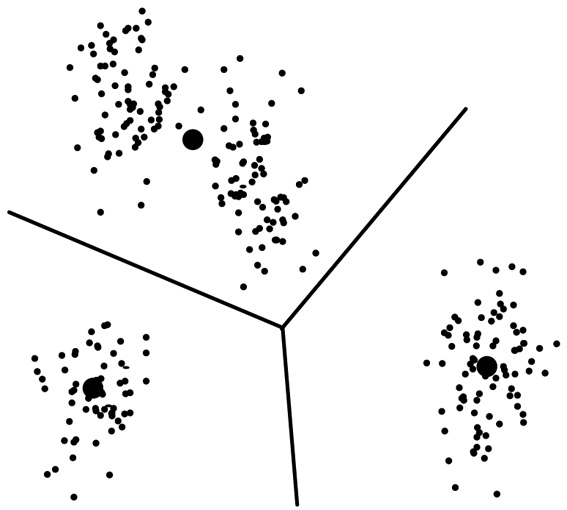
\includegraphics[width=5cm]{images/xmeans1.jpg}}\vspace{1mm}
  \subfloat[Selección punto de partida de K-Means ($k=2$).]{
   \label{f:step2}
    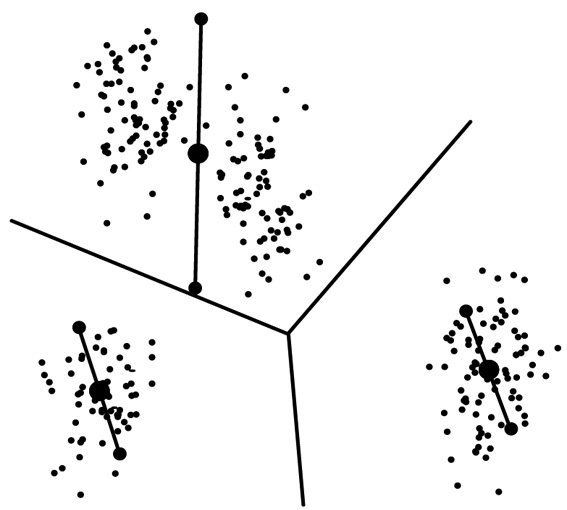
\includegraphics[width=5cm]{images/xmeans2.jpg}}\hspace{1mm}
  \subfloat[Resultado K-Means, evaluación BIC.]{
   \label{f:step3}
    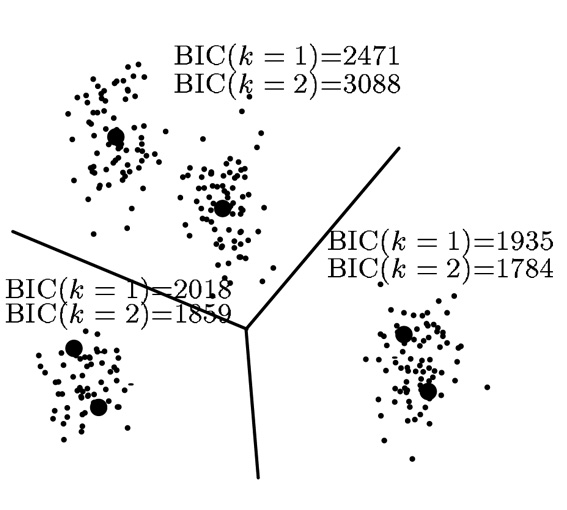
\includegraphics[width=5cm]{images/xmeans3.jpg}}\vspace{1mm}
  \subfloat[Resultado iteración X-Means]{
   \label{f:step4}
    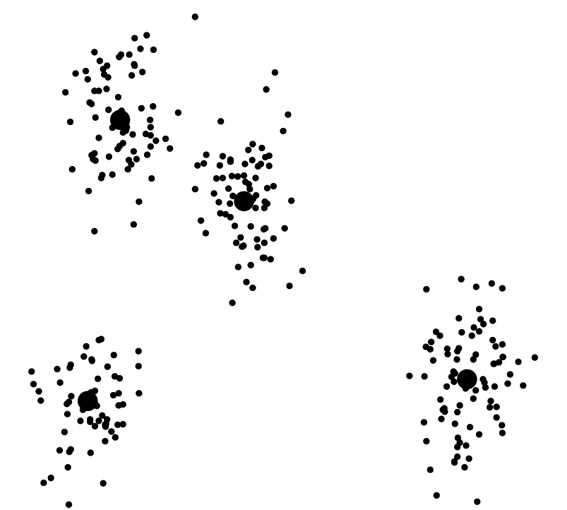
\includegraphics[width=5cm]{images/xmeans4.jpg}}
 \caption{Iteración X-Means.}
 \label{f:xmeans_steps}
\end{figure}

\subsection{Ventajas}

Una de las principales ventajas que posee este algoritmo radica en que es más escalable debido a que con cada iteración se reduce más el número de datos en los cuales K-Means se debe ejecutar, lo que hace que sea más fácil utilizarlo en conjuntos de datos de mayor tamaño. Otra ventaja es que se sabe que con K-Means de pocos clústers es menos probable incurrir en mínimos locales en comparación a uno realizado con muchos clústers. Por lo tanto, el hecho de que X-Means utilice un K-Means con $K=2$ favorece a que no se atasque en mínimos locales.

Además este método permite realizar una visualización del tipo árbol, la que crea una estructura jerárquica de los clústers.
%archivo implementacion
\chapter{Resultados y Análisis}

Una vez realizados los experimentos con el algoritmo de agrupamiento X-Means, se presentan los resultados en diferentes figuras y tablas. Primero se encuentran los resultados conseguidos al ejecutar el algoritmo con los atributos de las tablas \ref{tab:atributos_establecimientos} y \ref{tab:atributos_matriculas}, para ver cuales atributos son los mas importantes. Luego se presentan los resultados al comparar el mejor resultado de la etapa anterior con el resultado que se obtiene al agregarle las variables de relación establecimiento-matrícula.

\section{Resultados obtenidos}

La tabla \ref{tab:cl_estab} muestra los resultados al ejecutar X-Means sobre la base de datos de establecimientos en 3 diferentes ocasiones, diferenciándose por la cantidad de atributos que se utilizan. Una con todos los atributos, una con los de importancia alta y media, y finalmente una solo con los atributos de importancia alta.

Las siglas de los clústers de establecimientos sin considerar los atributos de relación establecimientos-matrícula (tablas \ref{tab:cl_estab}, \ref{tab:cl_atr_estab} y \ref{tab:cl_depe_estab}) corresponden a:

\begin{itemize}
    \item BCBM: Bajo Costo Baja Matricula (menor a 390 alumnos).
    \item BCAM: Bajo Costo Alta Matricula (sobre 700 alumnos).
    \item MCAM: Medio Costo Alta Matricula (sobre 700 alumnos).
    \item ACMM: Alto Costo Media Matrícula (entre 391 y 700 alumnos).
\end{itemize}

\begin{table}[H]
\centering
\caption{Clústers de establecimientos variando la cantidad de atributos (por grupos de importancia).}
\label{tab:cl_estab}
\begin{tabular}{|c|c|c|c|c|}
\hline
\textbf{Atributos} & \textbf{BCBM} & \textbf{BCAM} & \textbf{MCAM} & \textbf{ACMM}   \\ \hline
Todos & 959 & 826 & 247 & 36 \\ \hline
Alta + Media & 959 & 540 & 311 & 258 \\ \hline
Alta & 977 & 524 & 308 & 259\\ \hline
\end{tabular}
\end{table}

La tabla \ref{tab:cl_atr_estab} muestra los resultados obtenidos al ejecutar X-Means en los atributos de la base de datos de establecimientos (tabla \ref{tab:atributos_establecimientos}) con importancia alta.

\begin{table}[H]
\centering
\caption{Comparativa de clústers de establecimientos por atributo.}
\label{tab:cl_atr_estab}
\resizebox{\textwidth}{!}{\begin{tabular}{|l|l|l|l|l|}
\hline
& \textbf{BCBM} & \textbf{BCAM} & \textbf{MCAM} & \textbf{ACMM} \\ \hline
\textbf{Dependencia}                    & P.Subvencionado / Municipal & \begin{tabular}[c]{@{}l@{}}P. Subvencionado / Municipal / \\ Corp. Adm. Deleagada\end{tabular} & P. Subvencionado   & P. Pagado        \\ \hline
\textbf{Educación}               & Básica / Media              & Media / Completa                                                                               & Media / Completa   & Completa         \\ \hline
\textbf{Matrícula}               & Gratuita / Menor a \$25.000 & Gratuita / Menor a \$25.000                                                                    & Menor a \$10.000   & Mayor a \$50.000 \\ \hline
\textbf{Mensualidad}             & Gratuita / Menor a \$25.000 & Gratuita / Menor a \$25.000                                                                    & $25.000 - $100.000 & Mayor a \$50.000 \\ \hline
\textbf{Convenio SEP}            & Si                          & Si                                                                                             & No                 & No               \\ \hline
\textbf{Prom. matrículas}        & 383                         & 781                                                                                            & 905                & 686              \\ \hline
\textbf{Prom. alumnos por curso} & 26                          & 30                                                                                             & 32                 & 21               \\ \hline
\textbf{Prom. de becas}          & 19                          & 59                                                                                             & 91                 & 8                \\ \hline
\end{tabular}}
\end{table}

\begin{table}[H]
\centering
\caption{Clústers de establecimientos (tabla \ref{tab:cl_atr_estab}) según su dependencia.}
\label{tab:cl_depe_estab}
\begin{tabular}{|c|c|c|c|c|}
\hline
\textbf{Clúster} & \textbf{Municipal} & \textbf{P. Subvencionado} & \textbf{P. Pagado} & \textbf{Corp. Admin. Del.}   \\ \hline
BCBM & 485 & 491 & 1 & 0 \\ \hline
BCAM & 173 & 318 & 0 & 33 \\ \hline
MCAM & 3 & 303 & 2 & 0 \\ \hline
ACMM & 0 & 1 & 258 & 0 \\ \hline
\end{tabular}
\end{table}

En la tabla \ref{tab:cl_atr_estab_rel} se encuentran los resultados que se obtuvieron al ejecutar el algoritmo de agrupamiento en la base de datos conformada por los atributos de importancia alta de la tabla \ref{tab:atributos_establecimientos} y los atributos de relación establecimiento-matrícula de la tabla \ref{tab:atributos_relacion_establecimientos}.

Las siglas utilizadas para los clústers de establecimientos considerando los atributos de relación establecimientos-matrícula (tablas \ref{tab:cl_atr_estab_rel}, \ref{tab:cl_depe_estab_rel} y \ref{tab:cl_estab_sobre_edad}) corresponden a:
\begin{itemize}
    \item BCBMCD: Bajo Costo Baja Matricula (menor a 390 alumnos) Corta Distancia (menor a 4 km).
    \item BCAMMD: Bajo Costo Alta Matricula (sobre 700 alumnos) Media Distancia (entre 4 y 8 km).
    \item MCAMMD: Medio Costo Alta Matricula (sobre 700 alumnos) Media Distancia (entre 4 y 8 km).
    \item ACMMLD: Alto Costo Media Matrícula (entre 391 y 700 alumnos) Larga Distancia (sobre 8 km).
\end{itemize}

\begin{table}[H]
\centering
\caption{Comparativa de clústers de establecimientos por atributo, incluyendo los de relación establecimiento-matrícula.}
\label{tab:cl_atr_estab_rel}
\resizebox{\textwidth}{!}{\begin{tabular}{|l|l|l|l|l|}
\hline
& \textbf{BCBMPD} & \textbf{BCAMMD} & \textbf{MCAMMD} & \textbf{ACMMLD} \\ \hline
\textbf{Dependencia}                                                                  & P. Subvencionado / Municipal & \begin{tabular}[c]{@{}l@{}}P. Subvencionados / Municipales /\\ Corp. Adm. Delegada\end{tabular} & P. Subvencionado   & P. Pagado        \\ \hline
\textbf{Educación}                                                                    & Básica                       & Media / Completa                                                                                & Media / Completa   & Completa         \\ \hline
\textbf{Matrícula}                                                                    & Gratuita                     & Gratuita / Menor a \$25.000                                                                     & Menor a \$10.000   & Mayor a \$50.000 \\ \hline
\textbf{Mensualidad}                                                                  & Gratuita / Menor a \$25.000  & Gratuita / Menor a \$25.000                                                                     & $25.000 - $100.000 & Mayor a \$50.000 \\ \hline
\textbf{Convenio SEP}                                                                 & Si                           & Si                                                                                              & No                 & No               \\ \hline
\textbf{Prom. matrículas}                                                             & 383                          & 781                                                                                             & 895                & 686              \\ \hline
\textbf{Prom. alumnos por curso}                                                      & 26                           & 30                                                                                              & 32                 & 21               \\ \hline
\textbf{Prom. de becas}                                                               & 19                           & 58                                                                                              & 91                 & 8                \\ \hline
\textbf{IDE}                                                                          & 0,5 - 1                      & -0,5 - 0                                                                                        & 0 - 1,5            & 1 - 1,5          \\ \hline
\begin{tabular}[c]{@{}l@{}}\textbf{Distancia}\\ \textbf{Establecimiento - Hogar}\end{tabular} & 2,960 km                     & 5,204 km                                                                                        & 5,207 km           & 9,761            \\ \hline
\textbf{Sobre edad promedio}                                                                   & 0,524                        & 0,488                                                                                           & 0,297              & 0,488            \\ \hline
\end{tabular}}
\end{table}

\begin{table}[H]
\centering
\caption{Clústers de establecimientos (tabla \ref{tab:cl_atr_estab_rel}) según su dependencia.}
\label{tab:cl_depe_estab_rel}
\begin{tabular}{|c|c|c|c|c|}
\hline
\textbf{Clúster} & \textbf{Municipal} & \textbf{P. Subvencionado} & \textbf{P. Pagado} & \textbf{Corp. Admin. Del.}   \\ \hline
BCBMPD & 485 & 489 & 1 & 0 \\ \hline
BCAMMD & 173 & 307 & 0 & 33 \\ \hline
MCAMMD & 3 & 316 & 2 & 0 \\ \hline
ACMMLD & 0 & 1 & 258 & 0 \\ \hline
\end{tabular}
\end{table}

\begin{table}[H]
\centering
\caption{Detalle de la sobre edad en los clústers de establecimientos. }
\label{tab:cl_estab_sobre_edad}
\begin{tabular}{|l|c|c|c|c|c|}
\hline
                & \textbf{\% del total} & \textbf{\% 1 año\footnotemark} & \textbf{\% 2 años\footnotemark[\value{footnote}]\footnotemark[\value{footnote}]} & \textbf{\% 3 años\footnotemark[\value{footnote}]} & \textbf{\% 4 años\footnotemark[\value{footnote}]} \\ \hline
\textbf{BCBMPD} & 31                    & 74,8              & 18,9               & 5,2                & 1,1                \\ \hline
\textbf{BCAMMD} & 32,9                  & 75,1              & 20,5               & 3,9                & 0,5                \\ \hline
\textbf{MCAMMD} & 24                    & 85,3              & 13                 & 1,6                & 0,1                \\ \hline
\textbf{ACMMLD} & 38,1                  & 94,9              & 4,6                & 0,4                & 0,1                \\ \hline
\end{tabular}
\end{table}

\footnotetext{Porcentajes en base al total de alumnos con sobre edad mayor o igual a 1.}

Las siguientes tablas, y de manera similar a lo descrito anteriormente para los establecimientos, muestran los resultados obtenidos usando los datos de las matrículas. En la tabla \ref{tab:cl_mat} se muestran los resultados con los datos de la tabla \ref{tab:atributos_matriculas} en 3 diferentes versiones, según la importancia del atributo. La primera con todos los atributos, luego solo con los de alta y media, y finalmente solo los de alta importancia.

Las siglas utilizadas para los clústers de matrículas sin atributos de relación (tablas \ref{tab:cl_mat}, \ref{tab:cl_atr_mat} y \ref{tab:cl_mat_sobre_edad}) corresponden a:

\begin{itemize}
    \item MCB: Mujeres Con Beneficio.
    \item HCB: Hombres Con Beneficio.
    \item MSB: Mujeres Sin Beneficio.
    \item HSB: Hombres Sin Beneficio.
\end{itemize}

\begin{table}[H]
\centering
\caption{Clústers de matrículas variando la cantidad de atributos (por grupos de importancia).}
\label{tab:cl_mat}
\begin{tabular}{|c|c|c|c|c|}
\hline
\textbf{Atributos} & \textbf{MCB} & \textbf{HCB} & \textbf{MSB} & \textbf{HSB}   \\ \hline
Todos & 551932 & 442048 & 40803 & 13585 \\ \hline
Alta + Media & 551932 & 442048 & 34088 & 20300 \\ \hline
Alta & 286089 & 300007 & 230486 & 231786 \\ \hline
\end{tabular}
\end{table}

En las tablas \ref{tab:cl_atr_mat} y \ref{tab:cl_atr_mat_rel} se muestran primero los resultados obtenidos al utilizar los atributos de alta importancia de la tabla \ref{tab:atributos_matriculas} y luego los que se obtienen al incluir los atributos de relación de la tabla \ref{tab:atributos_relacion_matriculas}.

\begin{table}[H]
\centering
\caption{Comparativa de clústers de matrículas por atributo.}
\label{tab:cl_atr_mat}
\resizebox{\textwidth}{!}{\begin{tabular}{|l|l|l|l|l|}
\hline
& \textbf{MCB} & \textbf{HCB} & \textbf{MSB} & \textbf{HSB} \\ \hline
\textbf{Género}           & Femenino                                                                                                         & Masculino                                                                                                        & Femenino & Masculino \\ \hline
\textbf{Beneficiario SEP} & Si                                                                                                               & Si                                                                                                               & No       & No        \\ \hline
\textbf{Criterio SEP}     & \begin{tabular}[c]{@{}l@{}}Pertenece a Chile solidario / \\ Puntaje de ficha de protección\\ social\end{tabular} & \begin{tabular}[c]{@{}l@{}}Pertenece a Chile solidario / \\ Puntaje de ficha de protección\\ social\end{tabular} &          &           \\ \hline
\textbf{Sobre edad}       & 0,364                                                                                                            & 0,488                                                                                                            & 0,284    & 0,365     \\ \hline
\end{tabular}}
\end{table}


\begin{table}[H]
\centering
\caption{Detalle de la sobre edad en los clústers de matrículas.}
\label{tab:cl_mat_sobre_edad}
\begin{tabular}{|l|c|c|c|c|c|}
\hline
             & \textbf{\% del total} & \textbf{\% 1 año\footnotemark} & \textbf{\% 2 años\footnotemark[\value{footnote}]} & \textbf{\% 3 años\footnotemark[\value{footnote}]} & \textbf{\% 4 años\footnotemark[\value{footnote}]} \\ \hline
\textbf{MCB} & 28,5                  & 76,9              & 18,5               & 4                  & 0,6                \\ \hline
\textbf{HCB} & 36,4                  & 72,5              & 21,5               & 5,1                & 0,9                \\ \hline
\textbf{MSB} & 25,7                  & 90.2              & 8,7                & 1                  & 0,1                \\ \hline
\textbf{HSB} & 32                    & 87,3              & 11,1               & 1,5                & 0,1                \\ \hline
\end{tabular}
\end{table}

\footnotetext{Porcentajes en base al total de matrículas con sobre edad mayor o igual a 1.}

Las siglas utilizadas para los clústers de matrículas, incluyendo los atributos de relación, (tablas \ref{tab:cl_atr_mat_rel} y \ref{tab:cl_mat_rel_sobre_edad}) corresponden a:

\begin{itemize}
    \item MCBBC: Mujeres Con Beneficio Bajo Costo.
    \item HCBBC: Hombres Con Beneficio Bajo Costo.
    \item MiSBMC: Mixto Sin Beneficio Medio Costo.
    \item MiSBAC: Mixto Sin Beneficio Alto Costo.
\end{itemize}

\begin{table}[H]
\centering
\caption{Comparativa de clústers de matrículas por atributo, incluyendo los de relación  establecimiento-matrícula.}
\label{tab:cl_atr_mat_rel}
\resizebox{\textwidth}{!}{\begin{tabular}{|l|l|l|l|l|}
\hline
& \textbf{MCBBC} & \textbf{HCBBC} & \textbf{MiSBMC} & \textbf{MiSBAC} \\ \hline
\textbf{Género}                                                                      & Femenino                                                                                                        & Masculino                                                                                                       & Femenino / Masculino & Femenino / Masculino \\ \hline
\textbf{Beneficiario SE}P                                                            & Si                                                                                                              & Si                                                                                                              & No                   & No                   \\ \hline
\textbf{Criterio SEP}                                                                & \begin{tabular}[c]{@{}l@{}}Pertenece a Chile solidario /\\ Puntaje de ficha de protección\\ social\end{tabular} & \begin{tabular}[c]{@{}l@{}}Pertenece a Chile solidario /\\ Puntaje de ficha de protección\\ social\end{tabular} &                      &                      \\ \hline
\textbf{Sobre edad}                                                                  & 0,370                                                                                                           & 0,492                                                                                                           & 0,270                & 0,401                \\ \hline
\textbf{Matrícula que paga}                                                          & Gratuita                                                                                                        & Gratuita                                                                                                        & Gratuita             & Mayor a \$100.000    \\ \hline
\textbf{Mensualidad que paga}                                                        & Gratuita                                                                                                        & Gratuita                                                                                                        & $10.000 - $100.000   & Mayor a \$100.000    \\ \hline
\begin{tabular}[c]{@{}l@{}}\textbf{Distancia}\\ \textbf{Establecimiento - Hogar}\end{tabular} & 4,711 km                                                                                                        & 4,939 km                                                                                                        & 5,912 km             & 4,911 km             \\ \hline
\end{tabular}}
\end{table}

\begin{table}[H]
\centering
\caption{Detalle de la sobre edad en los clústers de matrículas, incluyendo atributos de relación.}
\label{tab:cl_mat_rel_sobre_edad}
\begin{tabular}{|l|c|c|c|c|c|}
\hline
                & \textbf{\% del total} & \textbf{\% 1 año\footnotemark} & \textbf{\% 2 años\footnotemark[\value{footnote}]} & \textbf{\% 3 años\footnotemark[\value{footnote}]} & \textbf{\% 4 años\footnotemark[\value{footnote}]} \\ \hline
\textbf{MCBBC}  & 28,9                  & 76,7              & 18,7               & 3,9                & 0,7                \\ \hline
\textbf{HCBBC}  & 36,7                  & 72,4              & 21,6               & 5,1                & 0,9                \\ \hline
\textbf{MiSBMC} & 23,4                  & 85,9              & 12,4               & 1,6                & 0,1                \\ \hline
\textbf{MiSBAC} & 38,1                  & 94,9              & 4,6                & 0,4                & 0,1                \\ \hline
\end{tabular}
\end{table}

\footnotetext{Porcentajes en base al total de matrículas con sobre edad mayor o igual a 1.}

\section{Análisis de los resultados}

En esta sección se analizan los diferentes resultados obtenidos y presentados anteriormente, comenzando con el análisis para los establecimientos y seguido por el de las matrículas.

Lo primero que se aprecia en la tabla \ref{tab:cl_estab}, es que para las 3 versiones el clúster BCBM agrupa casi un 50\% del total de los colegios, en donde además en la segunda y tercera versión el resto de los clústers presentan una cardinalidad similar. Esto demuestra que en este caso incluir variables consideradas de importancia media y baja no generan un gran impacto en el resultado final.

Teniendo en cuenta lo anterior, y de que por tratarse de un aprendizaje no supervisado es difícil establecer una medida de eficiencia, se consideró la tercera versión para el resto del estudio. Es decir, se tomará la versión en la cual solo se utilizaron los atributos clasificados como de alta importancia. Además se debe considerar que al ejecutar el algoritmo con menos variables el tiempo de ejecución es menor.

A partir de los resultados obtenidos para los establecimientos y de las figuras generadas con estos (figuras \ref{fig:radar_estab} y \ref{fig:radar_estab_rel}), podemos ver que al realizar una comparación entre ambas ejecuciones del algoritmo (sin y con atributos de relación) no se generan grandes cambios en los clústers, pero si aumenta el nivel de información y detalle de cada uno de ellos, incorporando nuevas características distintivas. Es por esto que el análisis se centrará en dichos resultados.

\begin{figure}[hc]
    \centering
    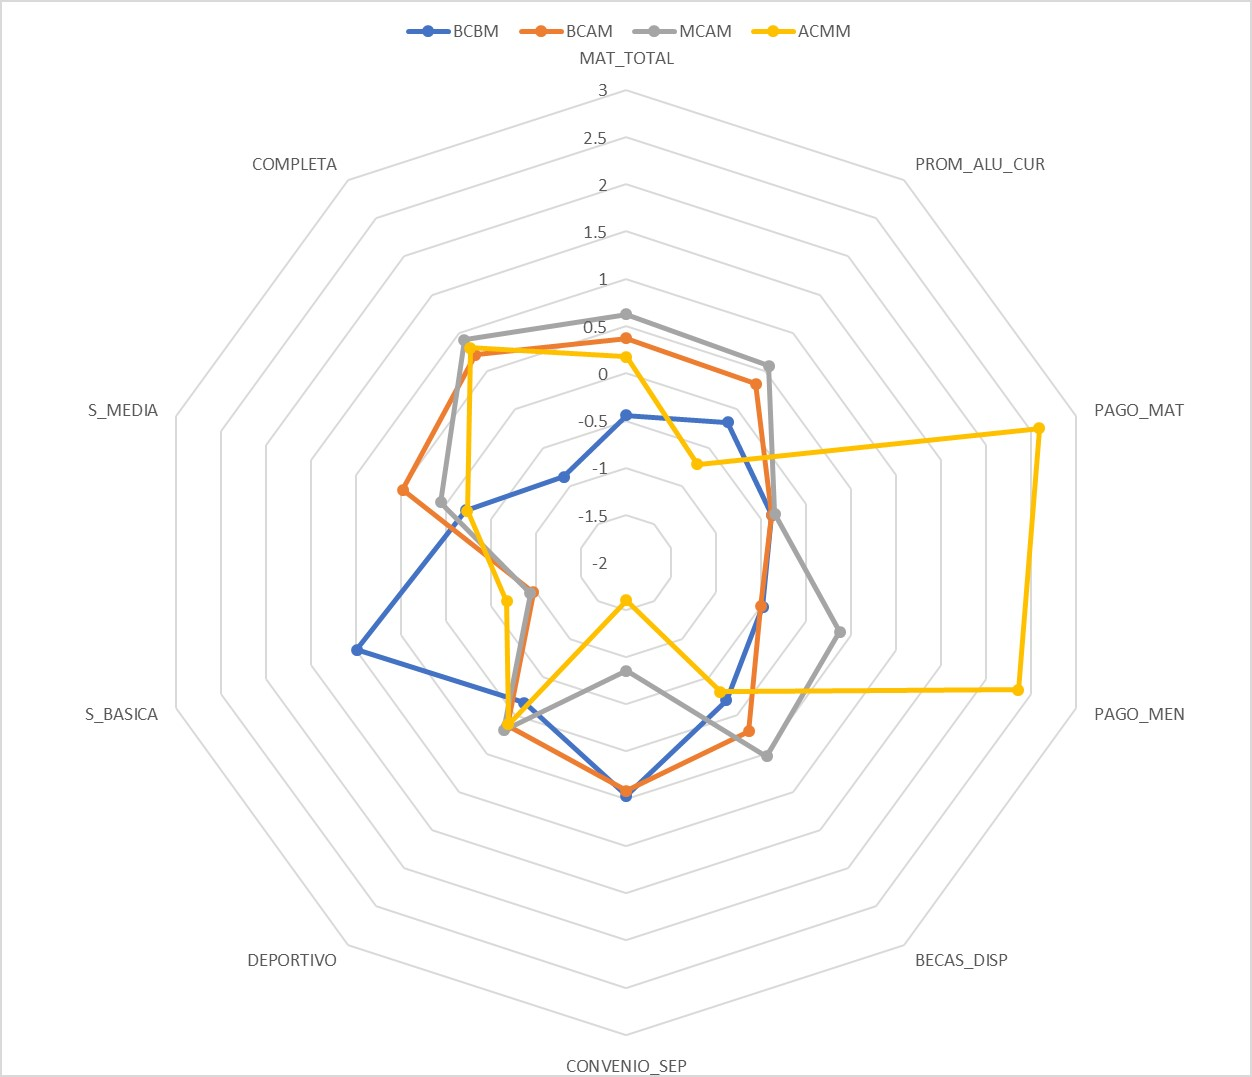
\includegraphics[width=0.66\textwidth]{images/radar_chart_establecimientos_sin.jpg}
    \caption{Promedios de atributos normalizados para establecimientos de la Región Metropolitana.}
    \label{fig:radar_estab}
\end{figure}

\begin{figure}[hc]
    \centering
    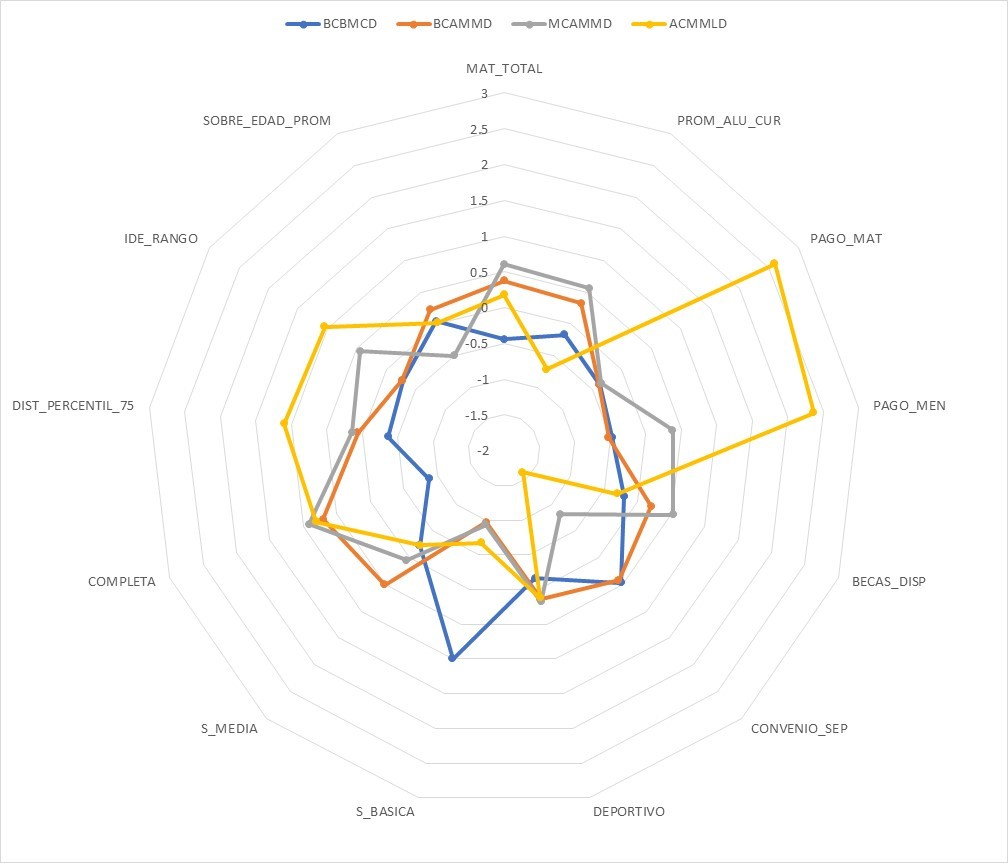
\includegraphics[width=0.66\textwidth]{images/radar_chart_establecimientos_con.jpg}
    \caption{Promedios de atributos normalizados de establecimientos con atributos relacionales (tabla \ref{tab:atributos_relacion_establecimientos}) de la Región Metropolitana.}
    \label{fig:radar_estab_rel}
\end{figure}

Los primeros dos clústers son colegios gratuitos o baratos con un IDE bajo que se diferencian entre ellos principalmente por el nivel de educación que imparten, en el primero predominan los de enseñanza básica y en el segundo establecimientos que imparten educación media o completa. El tercer y cuarto clúster se diferencia de los otros dos por tener un nivel de copago e IDE superiores, donde en el tercero se tienen valores medios y en el cuarto valores elevados. Por otro lado, al analizar la distancia que separa a los establecimientos de sus estudiantes, se aprecia notoriamente que el desplazamiento crece al aumentar el nivel del copago. Es decir, las familias que más pagan están dispuestas a desplazarse distancias mayores para llegar al establecimiento en comparación a familias que optan por colegios gratuitos o de bajo costo. Finalmente otro punto interesante de analizar es la sobre edad, que en el caso de los colegios más caros se concentra con un 95\% en un año de sobre edad. En el resto de los clústers el valor fluctúa entre un 75\% y 85\%, y el resto de distribuye de 2 a 4 años de sobre edad.

Para el caso de las matrículas lo primero que se debe analizar es la tabla \ref{tab:cl_mat}, en donde se aprecian los resultados de las 3 ejecuciones con los diferentes atributos, agrupados por su nivel de importancia. Se puede ver que las primeras dos ejecuciones generan clústers de cardinalidad muy similares, diferenciándose claramente con el tercer resultado, el cual presenta clústers de tamaños similares. La diferencia se en que los clústers de la última ejecución poseen atributos que describen de mejor manera los grupos, los cuales se van perdiendo al ir añadiendo atributos adicionales. 

Además de lo ya mencionado, es importante tener en cuenta que agregar más atributos a una base de datos de un total de 1.500.000 registros aproximadamente, provocará que el tiempo requerido para su ejecución aumenta significativamente. Por lo tanto, se analizarán más a fondo los resultados de la tercera ejecución y se utilizará para comparar con los resultados que se obtienen al agregar los atributos de relación.

\begin{figure}[hc]
    \centering
    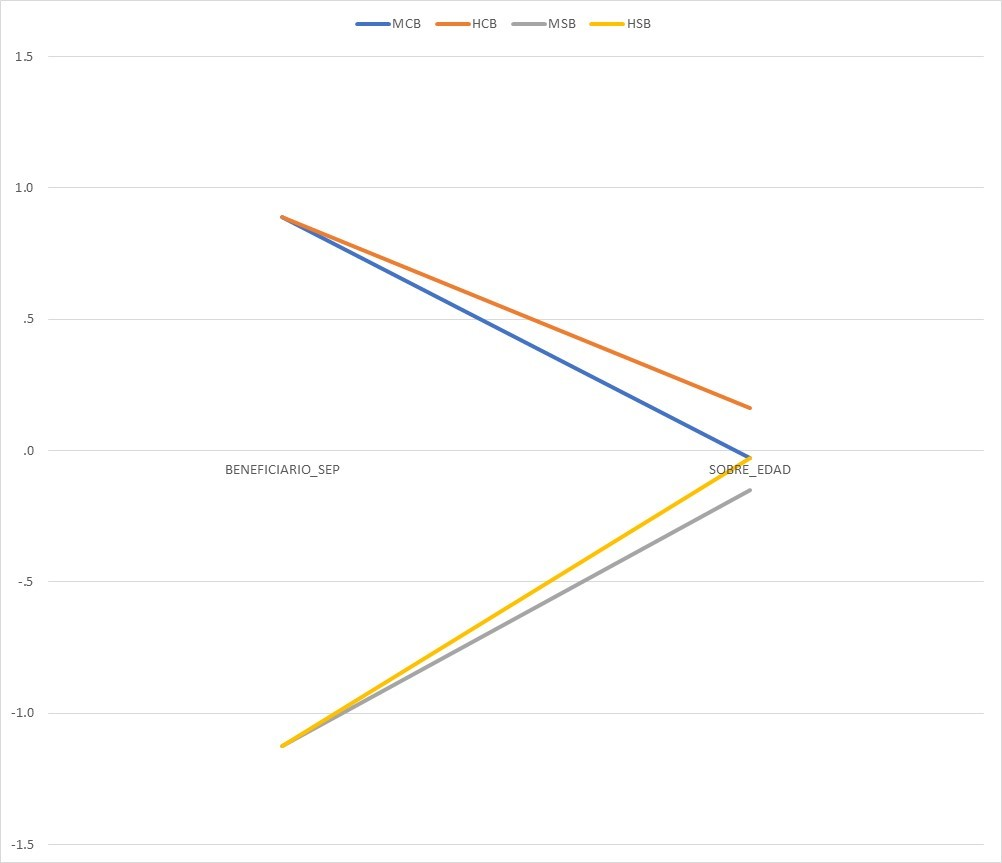
\includegraphics[width=0.66\textwidth]{images/chart_matriculas_sin.jpg}
    \caption{Promedio de atributos normalizados de matrículas de la Región Metropolitana.}
    \label{fig:chart_mat}
\end{figure}

\begin{figure}[hc]
    \centering
    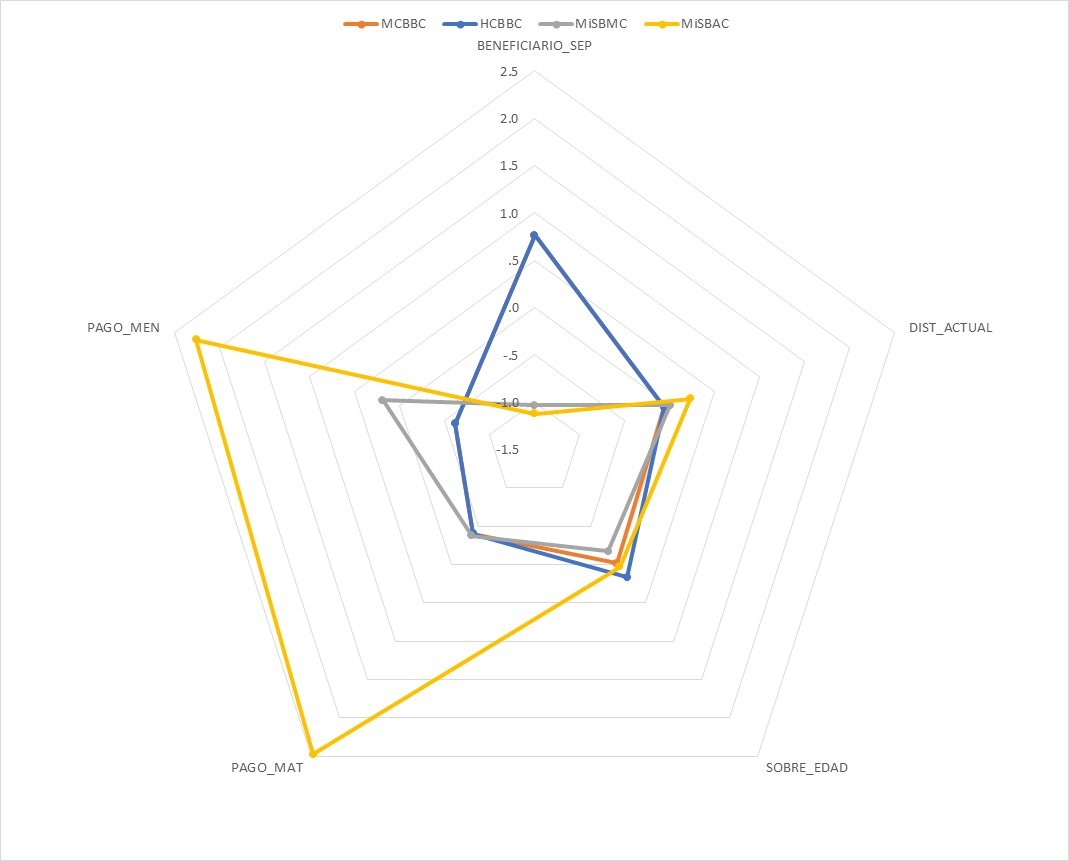
\includegraphics[width=0.66\textwidth]{images/radar_chart_matriculas_con.jpg}
    \caption{Promedio de atributos normalizados de matrículas con atributos relacionales (tabla \ref{tab:atributos_relacion_matriculas}) de la Región Metropolitana.}
    \label{fig:radar_mat_rel}
\end{figure}

Lo siguiente a analizar son las diferentes características de los clústers obtenidos para las matrículas y compararlos con los que se obtienen cuando se agregan los atributos de relación. Para facilitar la comparación entre clústers se generaron las figuras \ref{fig:chart_mat} y \ref{fig:radar_mat_rel}.
%fin desarrollo

%archivo conclusiones
\chapter*{Conclusiones}
\addcontentsline{toc}{chapter}{Conclusiones}




%archivo anexos
\renewcommand{\appendixname}{Anexos}
\renewcommand{\appendixtocname}{Anexos}
\renewcommand{\appendixpagename}{Anexos}

\appendix
\chapter{Anexo I}

\begin{longtable}{|p{5cm}|p{9cm}|}
\caption{Atributos seleccionados y generados para la base de datos de establecimientos.}\label{tab:atributos_establecimientos}\\
\hline
\endfirsthead
\caption[]{Atributos seleccionados y generados para la base de datos de establecimientos. (continuación)}\\
\hline
\endhead
\hline
\multicolumn{2}{|c|}{continúa $\ldots$}\\
\hline
\endfoot
\hline
\endlastfoot
\textbf{Atributo}  & \textbf{Descripción} \\ \hline
area\_metropolitana\_rbd & Pertenencia al área metropolitana. \\ \hline
cod\_depe & Código de dependencia del establecimiento. \\ \hline
gen\_rbd & Género del establecimiento. \\ \hline
mat\_total & Matrícula total de alumnos. \\ \hline
prom\_alu\_cur & Promedio de alumnos por curso. \\ \hline
pago\_mat & Nivel de pago de matrícula. \\ \hline
pago\_men & Nivel de pago de mensualidad. \\ \hline
becas\_disp & Becas disponibles en el establecimiento. \\ \hline
convenio\_sep & Posee convenio de subvención escolar preferencial (SEP). \\ \hline
deportivo & Nivel deportivo del establecimiento. \\ \hline
req\_papeles & Requisitos de papeles para postular. \\ \hline
req\_pruebas & Requisitos de prueba para postular. \\ \hline
req\_entrevista & Requisitos de entrevista para postular. \\ \hline
req\_pago & Requisitos de pago para postular. \\ \hline
req\_otros & Requisitos de cualquier tipo que no clasifique en las categorías anteriores. \\ \hline
enf\_académico & Enfoque académico. \\ \hline
enf\_valorico & Enfoque valórico. \\ \hline
enf\_laboral & Enfoque laboral. \\ \hline
enf\_otros & Enfoque de otro tipo que no clasifique en las categorías anteriores. \\ \hline
apoyo\_tutorias & Ofrece ayuda a los alumnos mediante tutorías. \\ \hline
apoyo\_especialistas & Ofrece ayuda a los alumnos mediante especialistas. \\ \hline
apoyo\_otros & Ofrece ayuda a los alumnos de cualquier otra forma que no clasifique en la categorías anteriores. \\ \hline
s\_basica & Establecimiento de enseñanza básica. \\ \hline
s\_media & Establecimiento de enseñanza media. \\ \hline
completa & Establecimiento de enseñanza completa. \\ \hline
IDE\_rango & Índice de desarrollo de la educación para todos por rango. \\ \hline
dist\_percentil\_75 & Distancia del percentil 75 de los alumnos que asisten al establecimiento. \\ \hline
\end{longtable} 

\chapter{Anexo II}

\begin{longtable}{|p{5cm}|p{9cm}|}
\caption{Atributos seleccionados y generados para la base de datos de matrículas.}\label{tab:atributos_matriculas}\\
\hline
\endfirsthead
\caption[]{Atributos seleccionados y generados para la base de datos de matrículas. (continuación)}\\
\hline
\endhead
\hline
\multicolumn{2}{|c|}{continúa $\ldots$}\\
\hline
\endfoot
\hline
\endlastfoot
\textbf{Atributo}  & \textbf{Descripción} \\ \hline
area\_metropolitana\_alu & Pertenencia al área metropolitana.\\ \hline
gen\_alu & Género del establecimiento. \\ \hline
area\_metropolitana\_alu & \\ \hline
cod\_sec & Código del sector económico.\\ \hline
cod\_espe & Código de especialidad. \\ \hline
cod\_rama & Código de rama. \\ \hline
grado\_sep & Corresponde a un nivel SEP.\\ \hline
beneficiario\_sep & Indicador del alumno beneficiario de la SEP.\\ \hline
criterio\_sep & Criterio por el cual se considera prioritario. \\ \hline
sobre\_edad & Diferencia entra la edad actual y la esperada para el nivel. \\ \hline
dist\_actual & Sitancia del alumno a su establecimiento actual\\ \hline
pago\_mat & Nivel de pago de matrícula. \\ \hline
pago\_men & Nivel de pago de mensualidad. \\ \hline
\end{longtable} 

\begin{table}[]
\centering
\caption{Resumen }
\label{my-label}
\begin{tabular}{|l|l|l|l|l|}
\hline
Año  & CIAE & MIME & \% de coincidencia   \\ \hline
2013 & 2110 & 2040 & 96,68 \\ \hline
2014 & 2095 & 2049 & 97,8  \\ \hline
2015 & 2088 & 2057 & 98,52 \\ \hline
2016 & 2068 & 2061 & 99,66 \\ \hline
\end{tabular}
\end{table}



%\backmatter
%\cleardoublepage

\singlespacing
\cleardoublepage

\bibliographystyle{plain}
\bibliography{bib/papers}

\end{document}